%%%% ijcai15.tex

% These are the instructions for authors for IJCAI-15.
% They are the same as the ones for IJCAI-11 with superficical wording
%   changes only.

\documentclass{article}
% The file ijcai15.sty is the style file for IJCAI-15 (same as ijcai07.sty).
\usepackage{ijcai15}
\usepackage[numbers]{natbib}
\usepackage{graphicx}
\usepackage{color}
%\usepackage{algorithmic}
\usepackage[]{algorithm2e}
\usepackage{hyperref}
\hypersetup{letterpaper,bookmarksopen,bookmarksnumbered,
pdfpagemode=UseOutlines,
colorlinks=true,
linkcolor=blue,
anchorcolor=blue,
citecolor=blue,
filecolor=blue,
menucolor=blue,
urlcolor=blue
}
\usepackage{subfigure}
\usepackage{booktabs}
\usepackage{latexsym,amssymb,amsmath} % for \Box, \mathbb, split, etc.
\newcommand{\stnote}[1]{\textcolor{blue}{\textbf{ST: #1}}}
\newcommand{\jgonote}[1]{\textcolor{green}{\textbf{JGO: #1}}}
\newcommand{\argmax}[1]{\underset{#1}{\operatorname{argmax}}\;}
\newcommand{\argmin}[1]{\underset{#1}{\operatorname{argmin}}\;}


% Use the postscript times font!
\usepackage{times}
\newcommand{\algorithmCTxt}{Ordered Confidence Bound}
\newcommand{\algorithmCFname}{OrderedConfidenceBound}

% the following package is optional:
%\usepackage{latexsym} 

% Following comment is from ijcai97-submit.tex:
% The preparation of these files was supported by Schlumberger Palo Alto
% Research, AT\&T Bell Laboratories, and Morgan Kaufmann Publishers.
% Shirley Jowell, of Morgan Kaufmann Publishers, and Peter F.
% Patel-Schneider, of AT\&T Bell Laboratories collaborated on their
% preparation.

% These instructions can be modified and used in other conferences as long
% as credit to the authors and supporting agencies is retained, this notice
% is not changed, and further modification or reuse is not restricted.
% Neither Shirley Jowell nor Peter F. Patel-Schneider can be listed as
% contacts for providing assistance without their prior permission.

% To use for other conferences, change references to files and the
% conference appropriate and use other authors, contacts, publishers, and
% organizations.
% Also change the deadline and address for returning papers and the length and
% page charge instructions.
% Put where the files are available in the appropriate places.

\title{Bandit-Based System Adaptation for Grasping}


\author{}

\begin{document}

\maketitle

\begin{abstract}
A key aim of current research is to create robots that can reliably
manipulate objects.  However, in many instances, information needed to
infer a successful grasp is latent in the environment and arises from
complicated physical dynamics; for example, a heavy object might need
to be grasped in the middle or else it will twist out of the robot's gripper.  
The contribution of this paper is an
approach for enabling a robot to learn models for 
localizing and grasping objects by formalizing a grasping system as an
n-armed bandit problem.  The robot performs best arm identification
using a variant of Hoeffding races that incorporates prior
information, enabling it to quickly find an optimal arm without
pulling all the arms as in UCB-based approaches.  We demonstrate that
our adaptation step significantly improves accuracy over a
non-adaptive system, enabling a robot to improve grasping
models through experience.


%%   To address this
%% problem, we focus not on {\em category-based} manipulation (pick up
%% any mug) but rather {\em instance-based} manipulation (pick up this
%% mug).  

%% Our framework runs on an unmodified Baxter
%% robot; using our algorithm, a robot can interact with an object for
%% twenty minutes, and then reliably and quickly localize it with vision
%% and pick it up with closed-loop visual servoing. 

%% Instance-based recognition and pose estimation can be highly
%% accurate but require the designer to adapt the system to the specific
%% object being manipulated in large and small ways, ranging from
%% collecting training data, to choosing parameter values, to selecting
%% algorithms for tasks such as image segmentation or bounding box
%% classification.  

\end{abstract}



\section{Introduction}
Robotics will assist us at childcare, help us cook, and provide
service to doctors, nurses, and patients in hospitals. Many of these
tasks require a robot to robustly perceive and manipulate objects in
its environment, yet robust object manipulation remains a challenging
problem.  Systems for general-purpose manipulation are computationally
expensive and do not enjoy high accuracy on novel
objects~\citep{saxena08}.  A common source of error is the presence of
latent dynamics that emerge from interactions between the object and
the robot's gripper.  For example, a heavy object might fall out of
the robot's gripper unless it grabs it close to the center.
Transparent or reflective surfaces that are not visible in IR or RGB
make it difficult to infer grasp points~\citep{x}.

To address these limitations, we propose an approach for enabling a
robot to learn about an object through exploration and adapt its
grasping model accordingly.  We frame the problem of model adaptation
as identifying the best arm for an n-armed bandit
problem~\citep{thompson33} where the robot aims to minimize simple
regret after a finite exploration period~\citep{bubeck09}.  Our robot
can obtain a high-quality reward signal (although sometimes at a
higher cost in time and sensing) by actively collecting additional
information from the environment.  Existing algorithms for best arm
identification require pulling all the arms as an initialization
step~\citep{mannor04, audibert10, chen14}, a prohibitive expense when
each arm pull takes on the order of 90 seconds and there are more than
1000 arms.  To address this problem, we present a new algorithm,
\algorithmCTxt, based on Hoeffding races~\citep{maron93}. In our
approach, the robot pulls arms in an order determined by a prior,
which allows it to try the most promising arms first. It can then
autonomously decide when to stop by bounding the confidence in the
result.

%% We use slower, more accurate sensing approaches
%% to provide supervision for faster, simpler methods that excel with
%% large amounts of training data.  For example, to perform grasping we
%% use an analytic model to select grasp points, but depending on the
%% object, the best grasp according to the analytic model may not be
%% optimal; the robot can learn better grasps for that object using the
%% analytic model as a prior and actively collecting data for that
%% object.

%%  a view-based model for closed-loop visual picking.  View-based
%% methods for instance detection have many advantages over methods using
%% 3D models, because they directly capture the visual appearance of the
%% object, and are relatively simple and efficient to implement because
%% they operate on low-level features~\citep{hsiao13}.  However these
%% systems require large amounts of training data for robust performance,
%% for example more than 2000 images which must be manually collected and
%% annotated with bounding boxes for the state of the art LINE2D
%% method~\citep{hinterstoisser12}.  Moreover, for manipulation,
%% view-based methods do not propose potential grasps, and autonomous
%% methods for recognizing visual grasps are prone to error. 

%% To address these issues, we present an approach for enabling a robot
%% to train its own view-based model to recognize and manipulate the
%% specific objects it will need to use during collaborations with
%% humans.  Using our algorithm, the robot detects candidate objects for
%% training using a depth sensor, then actively collects view-based
%% visual templates to perform robust instance-based object detection,
%% pose estimation and closed-loop grasping using visual servoing.
%% Because our camera can move with seven degrees of freedom, the robot
%% can collect large quantities of data leading to simple visual models
%% that perform with high accuracy even under occlusion.  Our approach is
%% enabled by three innovations: our end-to-end algorithm for collecting
%% view-based training data with supervision obtained from a
%% higher-reliability depth sensor, which is supported by a simple and
%% robust method for determining candidate grasps using a depth sensor
%% mounted on a seven-degree-of-freedom arm, along with an approach for
%% autonomously and reliably finding object bounding boxes once the
%% object is on a background such as a floor or table.


Our evaluation, performed on a Baxter robot, demonstrates that our
adaptation step improves the overall pick success rate from 55\% to
75\% on our test set of 30 household objects, shown in
Figure~\ref{fig:object_glory_shot}.  Moreover, our approach also
enables the robot to learn success probabilities for each object it
encounters; when the robot fails to infer a successful grasp for an
object, it knows this fact, enabling it to take active steps to
recover such as asking for help~\citep{tellex14}.

We first give an overview of our object detection and localization,
then formalize our grasping framework as a bandit problem, where each
arm corresponds to a grasp point on the object.
Section~\ref{sec:evaluation} describes our evaluation in simulation
and on the real robot with $30$ household objects,
Section~\ref{sec:relatedwork} covers related work, and
Section~\ref{sec:conclusion} concludes.

\begin{figure}
\subfigure[Before learning.]{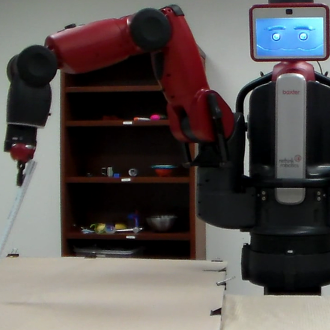
\includegraphics[width=0.5\linewidth]{figures/dropping_ruler.png}}%
\subfigure[After learning.]{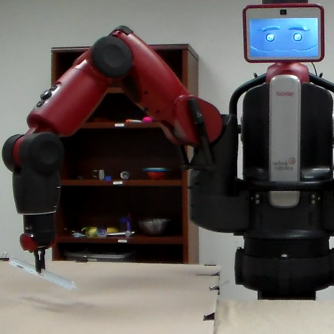
\includegraphics[width=0.5\linewidth]{figures/holding_ruler.png}}
\caption{Before learning, the robot grasps the ruler near the end, and it twists out of its gripper and falls onto the table when it lifts; after learning, the robot knows to grasp it near the center of mass.\label{fig:ruler}}
\end{figure}

%% Our software is compatible with ROS and the Baxter SDK version 1.0.0,
%% and we intend to release it as free software should our paper be
%% accepted.  As more and more instance-based models are collected, this
%% corpus will form a unique training set for category-based models for
%% detecting and grasping novel objects, since the robot will have a very
%% large number of views of a large set of objects as well as storing
%% depth information and grasping success.

\section{Object Detection and Localization}

The robot uses its arm cameras and IR sensor to localize objects in
the environment.  Our object detection and pose estimation pipeline
uses conventional computer vision algorithms to achieve a simple
software architecture, and a frame rate of about 2Hz for object
detection and pose estimation.  Our recognition pipeline takes video
from the robot, proposes a small number of candidate object bounding
boxes in each frame, and classifies each candidate bounding box as
belonging to a previously encountered object class. Our object classes
consist of object instances rather than pure object categories.  Using
instance recognition means we cannot reliably detect categories, such
as ``mugs,'' but the system will be able to detect, localize, and
grasp the specific instances for which it has models with much higher
speed and accuracy.  A visualization of data flow in the pipeline
appears in Figure~\ref{fig:system}.  For each module, we formalize its
input, output, and reward function; each component can have multiple
implementations which better for different objects.  The following
sections describe how we can use this pipeline to learn which
implementation to use for specific objects; this learning dramatically
speeds up performance.


\section{Bandit-based Adaptation}

Our formal model of a system defines a reinforcment learning problem,
in which the action space consists of different settings for system
parameters, and the reward function consists of the output of the
testing modules for each component.  The modular design of our system
supports a decomposition in the RL problem, so that we can treat each
optimization problem as a separate N-armed bandit problem.  In many
systems, the problem with this formulation is obtaining a reward
function to test different parameter values: the behavior of the
system must be measured by a person, and if an autonomous approach
existed to produce accurate output, it would obviate the need for the
system in the first place.  In contrast, in the robotic domain, many
edges in the system diagram can be verified, at the cost of time or
additional sensing.  This technique enables us to obtain high-quality
supervision at relevant edges in the system diagram, supporting the
decomposition into a bandit problem.  For example, optimizing grasp
height at level one is rewarded based on its accuracy at identifying
bounding boxes for the object; this training step does not require
running the entire pipeline.  Thus our algorithm for adaptation runs
from the root to the leaves of the system diagram, optimizing each
parameter based on the tester closest to it in the system tree.

Formally, the agent is given an n-armed bandit, where each arm pays
out $1$ with probability $\mu_i$ and $0$ otherwise.  The agent's goal
is to identify a good arm (with payout $>= k$) with probability $c$
(e.g., 95\% confidence that this arm is good) as quickly as possible.
As soon as it has done this, it should terminate.  The agent is also
given an ordering on the arms, promising ones first.  This order
corresponds to a prior, but the agent is only required to specific
that promising arms are first, not assign any specific probability
distribution on $\mu$.


Our algorithm, \algorithmCTxt, iterates through each arm, and try it
until we have identified it either is above $k$ with probability $c$
(in which case it terminates) or it is below $k$ with probability $c$
(in which case it moves to the next arm in the sequence.  To compute
this probability we need to estimate the probability that the true
payout probability, $\mu$ is greater than the threshold, $c$ given the
observed number of successes and failures:
\begin{align}
\Pr(\mu_i > c|  S, F)
\end{align}

We can compute this probability using the law of total probability:
\begin{align}
\Pr(\mu_i > c|  S, F) &= \int_k^1 \Pr(\mu_i=\mu | S, F) d\mu\\
\intertext{We assume a beta distribution on $\mu$:}
                      &= \int_k^1 \mu^S (1- \mu) ^F d\mu
\end{align}

This integral is the CDF of the beta distribution, and is called the
regularized incomplete beta function~\citep{olver10}. 

\begin{algorithm}
\SetKwFunction{x}{\algorithmCFname}
\x{$armOrder$, $k$, $\delta_{accept}$, $\delta_{reject}$}

$\mbox{Initialize } S_0 \dots S_n \mbox{ to } 0$\\
$\mbox{Initialize } F_0 \dots F_n \mbox{ to } 0$\\
\For {$i \in armOrder$}{
  $r \gets sample(arm_i)$\\
  \uIf {$r = 1$}{
    $S_i  \gets S_i + 1$
  }\uElse{
    $F_i  \gets F_i + 1$
  }
  $p_{below} \gets \int_0^k \Pr(\mu_i = \mu | S_i, F_i) d\mu $\\
  $p_{above} \gets \int_k^1 \Pr(\mu_i = \mu | S_i, F_i) d\mu $\\ %1 - p_{below}$\\
  $p_{threshold} \gets \int_{k - \epsilon}^{k + \epsilon} \Pr(\mu_i = \mu | S_i, F_i) d\mu $\\

  \uIf{$p_{above} \ge  \delta_{accept}$}{
    return $i$ \tcp*[r]{accept this arm}
  }\uElseIf{$p_{threshold} \ge \delta_{accept}$}{
    return $i$ \tcp*[r]{accept this arm}
  }\uElseIf{$p_{below} \ge \delta_{reject}$}{
    break \tcp*[r]{go to the next arm}
  } \Else{
    pass \tcp*[r]{keep pulling this arm}
  }
}

\caption{Ordered confidence bound algorithm for Best Arm
  Identification\label{alg:bandit}}
\end{algorithm}

Note that if $\mu = k$ the runtime is unbounded, so we fix an
$\epsilon > 0$ and accept a grasp if $\mu \in [k-\epsilon, k+\epsilon]$
with probability $c$.

This formalization gives rise to our policy, \algorithmCTxt, which
appears in Algorithm~\ref{alg:bandit}.    


%% * terminate fast, and know when to terminate
%% * identify the best grasp with high probability (and search longer if you haven't)
%% * providing a prior
%% * providing a bound on mu. 




\section{Robotic Implementation}

We use stock Baxter and one computer.  We use the wrist cameras to
obtain RGB at 30Hz.  The full visual system runs at 2Hz in typical
conditions.  We collect many measurements for the depth map by
performing an overhead raster scan of the object. The IR sensor
reports at about 30Hz but gives fairly good localization.  In order to
use the good resolution despite the sparsity of measurement induced by
the frequency of the sensor and the speed of the robot's movement, we
employ a Parzen kernel density estimator to record measurements at 1mm
resolution. We then downsample to 1cm resolution, which gives a very
clean map and a tractable state space for grasp inference.

%To obtain the 3D point cloud maps, we use the IR sensor in
%conjunction with the RGB camera.


%% The IR sensor is a triangulation rangefinder, which means it actively
%% illuminates its target with an infrared LED. If the robot is totally
%% deprived of light, the spot of light projected by the IR LED can be
%% seen in the RGB camera image. The location of the point in the image
%% changes significantly with the range of the point being measured. We
%% record the location at several reference ranges and interpolate
%% between the two closest reference points, allowing us to know the
%% pixel in the RGB image corresponding to the $(x,y,z)$ point being
%% measured. Together, this forms an $(r,g,b,x,y,z)$ measurement for the
%% pointcloud.


 
\section{Evaluation}
\label{sec:evaluation}

\begin{figure}
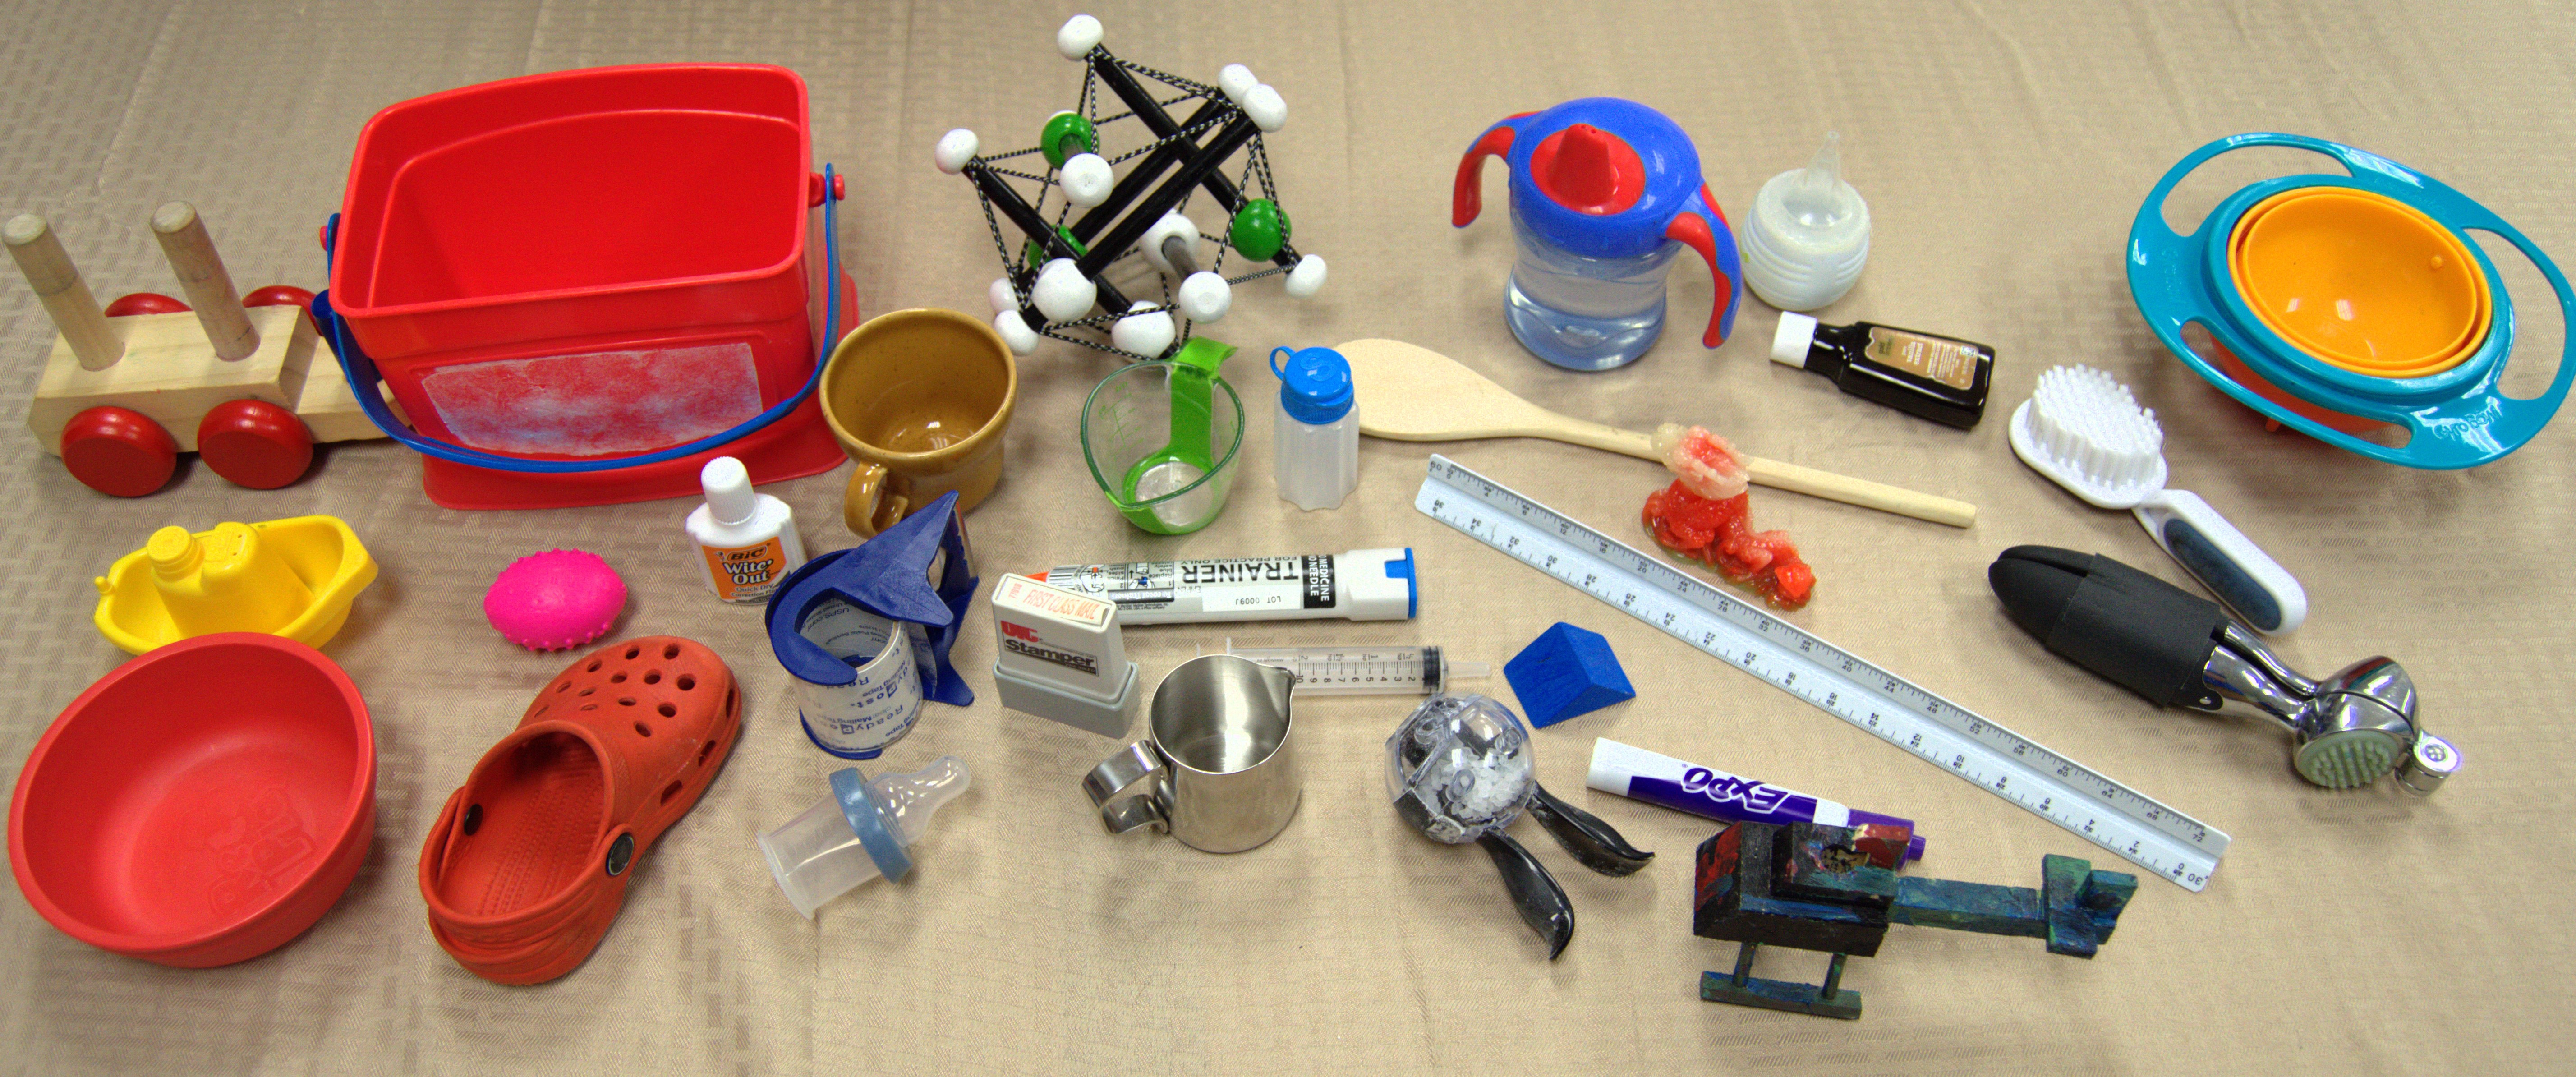
\includegraphics[width=1\linewidth]{figures/object_glory_shot.jpg}
\caption{The objects used in our evaluation.\label{fig:object_glory_shot}}
\end{figure}


The aim of our evaluation is to assess the ability of the system to
acquire visual models of objects which are effective for grasping and
object detection.  We first assess our approach in simulation,
comparing it to Thompson sampling and a fixed policy.  Next we
describe our robotic evaluation and manipulation which assesses our
system's ability to learn and adaptively improve its ability to grasp
objects, end-to-end.

\subsection{Simulation}

Our simulated results compare our approach to Thompson sampling as
well as a fixed policy, assessing the tradeoffs inherent in our choice
of parameters and algorithm.  We present results in
Table~\ref{fig:simulation_results}.  We simulate picking performance
by creating a sequence of $20$ bandits, where each arm pays out at a
rate of $0.1$ except for one, which pays out at $0.9$.  We move the
location of the best arm to a uniformly sampled random position in the
sequence.
\begin{figure}
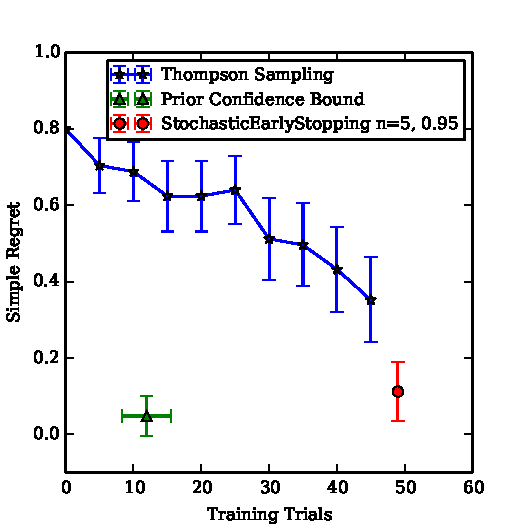
\includegraphics{figures/bestarm.pdf}
\caption{Results comparing our approach to various baselines in simulation.\label{fig:simulation_results}}
\end{figure}


\subsection{Robotic Evaluation}
 We have implemented our approach on the Baxter
robot, which is equipped with a seven-degree-of-freedom arm with a
camera and IR depth sensor, which we use as a one-pixel depth camera
to acquire our models.

The robot acquired visual and RGB-D models for N objects using our
autonomous learning system.  We manually verified that the scans were
accurate, and set the following parameters: height above the object
for the IR scan (to approximately 2cm); this height could be acquired
automatically by doing a first coarse IR scan following by a second IR
scan 2cm above the tallest height, but we set it manually to save
time.  Additionally we set the height of the arm for the initial servo
to acquire the object.

After acquiring visual and IR models for the object at different poses
of the arm, the robot performed the bandit-based adaptation step using
Algortihm~\ref{alg:bandit}.

We report the performance of the robot at picking using the learned
height for servoing, but without grasp learning, then the number of
trials used for grasp learning by our algorithm, and finally the
performance at picking using the learned grasp location.

After the robot detects an initially successful grab, we have it
shake the object vigorously to ensure that it would not fall out during
transport. After releasing the object and moving away, the robot checks 
to make sure the object is not stuck in its gripper. If the object
falls out during shaking or does not release properly, the grasp is
recorded as a failure. If the object is stuck, the robot pauses and
requests assistance before proceeding.

Most objects have more than one pose in which they can stand upright on
the table. If the robot knocks over an object, the model taken in the 
reference pose is no longer meaningful. Thus, during training,
we monitored the object and returned it to the reference pose whenever the 
robot knocked it over. Future work will incorporate multiple components in
the models which will allow the robot to cope with objects whose pose
can change during training. 

Our algorithm used an accept threshold of $0.7$, reject confidence of
$0.95$ and epsilon of $0.2$.  These parameters result in a policy that
rejects a grasp after one failed try, and accepts if the first three
picks are successful.  Different observations of success and failure
will cause the algorithm to try the grasp more to determine the true
probability of success.  The policy for exploring an arm appears in
Figure~\ref{fig:policy}.

\begin{figure}
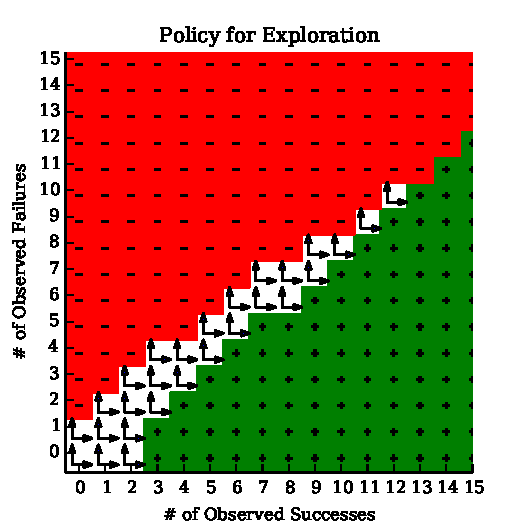
\includegraphics{figures/policy.pdf}
\caption{Policy for the agent given a belief state, defined by an
  observed number of succeseses and failures on that arm for our model
  parameters.  Red (-) shows states where the agent rejects the arm
  and move to the next one; green (+) shows states where it accepts
  the arm and stops learning, and the arrows show movement to the next
  belief state based on whether the next trial is successful.}
\end{figure}

\begin{table}
\small
\begin{tabular}{cccc}
\toprule
		    & Prior         &  Training     & Marginal\\
\midrule
\multicolumn{4}{c}{$\delta = 0; training = 3$} \\
\midrule
% too easy
Brush    	    & 10/10         &  3/3         &  10/10\\
Packing Tape        & 9/10          &  3/3         &  9/10 \\
Purple Marker       & 9/10          &  3/3         &  9/10 \\
Red Bowl    	    & 10/10         &  3/3         &  10/10\\
Red Bucket    	    & 5/10          &  3/3         &  5/10 \\
Shoe    	    & 10/10         &  3/3         &  10/10\\
Stamp    	    & 8/10          &  3/3         &  8/10 \\
Whiteout    	    & 10/10         &  3/3         &  10/10\\
Wooden Spoon        & 7/10          &  3/3         &  7/10 \\
% good improvement  
\midrule
\\
\multicolumn{4}{c}{$\delta >= 2$} \\
\midrule
Big Syringe    	    & 1/10          &  13/50       &  4/10 \\
Blue Salt Shaker    & 6/10          &  5/10        &  8/10 \\
Bottle Top    	    & 0/10          &  5/17        &  7/10 \\
Garlic Press        & 0/10          &  8/50        &  2/10 \\
Gyro Bowl    	    & 0/10          &  5/15        &  3/10 \\
Metal Pitcher       & 6/10          &  7/12        &  10/10\\
Mug    		    & 3/10          &  3/4         &  10/10\\
Round Salt Shaker   & 1/10          &  4/16        &  9/10 \\
Sippy Cup    	    & 0/10          &  6/50        &  4/10 \\
Triangle Block      & 0/10          &  3/13        &  7/10 \\
Vanilla	   	    & 5/10          &  4/5         &  9/10 \\
Wooden Train        & 4/10          &  11/24       &  8/10 \\

\midrule
\\
\multicolumn{4}{c}{$\delta <= 1$} \\
\midrule
% little to no improvement
Clear Pitcher       & 4/10          &  3/4         &  4/10 \\
Dragon    	    & 8/10          &  5/6         &  7/10 \\
Epipen    	    & 8/10          &  4/5         &  8/10 \\
Helicopter    	    & 2/10          &  8/39        &  3/10 \\
Icosahedron    	    & 7/10          &  7/21        &  8/10 \\
Ruler    	    & 6/10          &  5/12        &  7/10 \\
Syringe    	    & 9/10          &  6/9         &  10/10\\
Toy Egg    	    & 8/10          &  4/5         &  9/10 \\
Yellow Boat    	    & 9/10          &  5/6         &  9/10 \\
\midrule
Total		    & 165/300       &  148/400     & 224/300\\
Rate		    & 0.55          &  0.37        & 0.75\\
\bottomrule
\end{tabular}
\caption{Results from the robotic evaluation. We tested on 30 objects. The top block
contains objects which succeeded on the initial grasp estimate and therefor did not
learn a new grasp. The middle block contains objects which spent some time learning
and improved their performance notably. The bottom block contains objects for which 
some learning occurred but little or more improvement was seen. A performance
drop after learning was seen on one class: Dragon.\label{table:robot_results}}
% Curses to the dragon. Curses to Smaug!
% jgo: I double and triple checked the sums.
\end{table}

\subsection{Discussion}
Consider the top block in Figure~\ref{fig:robot_results}, the objects for which the
initially estimated grasp succeeds 3 times in a row. Note that when 10 trials are performed,
the variance in performance is about what we would expect.

% XXX TODO
% talk about successes and failures
The first few grasps suggested by the prior for the Triangle Block were infeasible because
the gripper slid over the sloped edges and pinched the block out of its grippers. The robot
tried grasps until it found one that targeted the sides that were parallel to the grippers,
resulting in a flush grasp.

For the Round Salt Shaker, the robot first attempted to grab the round plastic dome, which 
is infeasible. It tried grasps until it found one on the handle.

The Garlic Press is a geometrically simple object but quite heavy compared to the others. The
robot found a few grasps which might have been good for a lighter object, but it frequently
shook the press out of its grippers when confirming grasp quality.

The Big Syringe has some good grasps which are detected well by the prior, but due to its poor
contrast and transparent tip, orientation servoing was imprecise and the robot was unable to
learn well due to poor signal. What improvement did occur was due to finding a grasp which
consistently deformed the bulb into a grippable shape regardless of the perceived orientation
of the syringe. Similar problems were observed with the Clear Pitcher and Icosahedron.

Some of the objects had several grasps of similar, mediocre quality, which
caused the robot to try multiple grasps several times, eventually accepting one of the
mediocre grasps by chance.

The Red Bucket exhibited interesting behavior. Its gradient profile is rectangular, but at the
chosen height only two opposing sides are visible. Due to symmetry it was able to find a good
grasp despite the degeneracy in the model. Most of its failures were because the object is tall
and the robot did not back up enough before checking if the gripper was empty, which triggered
false negatives for grasp release.

Finally, some objects, such as the Helicopter and Dragon, barely fit in the gripper and would
therefor benefit from additional servo iterations to increase localization precision. 

\section{Related Work}

\label{sec:relatedwork}

\citet{bohg13} survey data-driven approaches to grasping.  Our
approaches can be thought of as a pipeline for automatically building
an experience database consisting of object models and known good
grasps, using analytic approaches to grasping unknown objects to
generate a grasp hypothesis space and bandit-based methods for trying
grasps and learning instance-based distributions for the grasp
experience database.  In this way our system achieves the best of both
approaches: models for grasping unknown objects can be applied; when
they do fail, the system can automatically recover by trying
grasps and adapting itself based on that specific object. Additionally, we
can use other grasp detectors to seed our prior, since it is only based
on an ordering and does not require an explicit probability distribution.
We can also interface with manual labeling similar to the forklift demarcation:
circle an area and we will restrict exploration to that region.

\citet{ude12} described an approach for detecting and manipulating
objects to learn models.  It uses a bag of words model and learns to
detect the objects.  It does not learn a model for grasping.
\citet{schiebener13} describes an extension that also does model
learning.  The robot pushes the object and then trains an object
recognition system.  It does not use a camera that moves and does not
grasp.
\citet{schiebener12} discovers and grasps unknown objects.

Summary: 
\begin{itemize}
\item People doing SLAM.  \citet{wang07, gallagher09}, 
\item People doing 3d reconstruction.   \citet{krainin11, banta00}
\item People doing big databases for category recognition.  \citet{kent14a, kent14, lai11a, goldfeder09}
\item Object tracking in vision (typically surveillance).
\item POMDPs for grasping.  \citet{platt11, hsiao10}
\item People doing systems.  \citet{hudson12, ciocarlie14}
\end{itemize}




Crowd-sourced and web robotics have created large databases of objects
and grasps using human supervision on the web~\citep{kent14a, kent14}.
These approaches outperform automatically inferred grasps but still
require humans in the loop.  Our approach enables a robot to acquire a
model fully autonomously, once the object has been placed on the
table.

\citet{zhu14} created a system for detecting objects and estimating
pose from single images of cluttered objects.  They use KinectFusion
to construct 3d object models from depth measurements with a
turn-table rather than automatically acquiring models.

\citet{chang12} created a system for picking out objects from a pile
for sorting and arranging but did not learn object models.  

next-best view planning~\citep{kriegel11}

\citet{nguyen14} learn to manipulate objects such as a light switch or
drawer with a similar self-training approach.  Our work learns visual
models for objects for autonomous pick-and-place rather than to
manipulate objects.

Developmental/cognitive robotics~\citep{lyubova13, kraft10r}

\citet{banta00} constructs a prototype 3d model from a minimum number
of range images of the object.  It terminates reconstruction when it
reaches a minimum threshold of accuracy.  It uses methods based on the
occluded regions of the reconstructed surfice to decide where to place
the camera and evaluates based on the reconstruction rather than pick
up success.  \citet{krainin11} present an approach for autonomous
object modeling using a depth camera observing the robot's hand as it
moves the object.  This system provides a 3d construction of the
object autonomously.  Our approach uses vision-based features and
evaluates based on grasp success.  Eye-in-hand laser
sensor.~\citep{aeotti14}

\stnote{Need to find the instance-based work that Erik mentioned when
  he said it was a ``solved problem.''}

\citet{velez11} created a mobile robot that explores the environment
and actively plans paths to acquire views of objects such as doors.
However it uses a fixed model of the object being detected rather than
updating its model based on the data it has acquired from the
environment.

Methods for planning in information space \citep{he08, atanasov13,
  prentice09} have been applied to enable mobile robots to plan
trajectories that avoid failures due to inability to accurately
estimate positions.  Our approach is focused instead on
object detection and manipulation, actively acquiring data for use
later in localizing and picking up objects. \stnote{May need to say
  more here depending on what GRATA actually is.}


Early models for pick-and-place rely on has been studied since the
early days of robotics~\citep{brooks83, lozano89}.  These systems
relied on models of object pose and end effector pose being provided to the
algorithm, and simply planned a motion for the arm to grasp.  Modern
approaches use object recognition systems to estimate pose and object
type, then libraries of grasps either annotated or learned from
data~\citep{saxena08, goldfeder09, morales03}.  These approaches
attempt to create systems that can grasp arbitrary objects based on
learned visual features or known 3d configuration.  Collecting these
training sets is an expensive process and is not accessible to the
average user in a non-robotics setting.  If the system does not work
for the user's particular application, there is no easy way for it to
adapt or relearn.  Our approach, instead, enables the robot to
autonomously acquire more information to increase robustness at
detecting and manipulating the specific object that is important to
the user at the current moment.

Visual-servoing based methods~\citep{chaumette06} \stnote{Need a whole
  paragraph about that. }

\stnote{\citet{ciocarlie14} seems highly relevant, could not read from
  the train's wifi.}  Existing work has collected large database of
object models for pose estimation, typically curated by an
expert~\citep{lai11}.  \citet{kasper12} created a semiautomatic system
that fuses 2d and 3d data, but the setup requires a special rig
including a turntable and a pair of cameras.  Our approach requires an
active camera mounted on a robot arm, but no additional equipment, so
that a robot in the home can autonomoulsy acquire new models.

\citet{collect14} describes an approach for lifelong robotic object
discovery, which infers object candidates from the robot's perceptual
data.  This system does not learn grasping models and does not
actively acquire more data to recognize, localize, and grasp the
object with high reliabilitiy.  It could be used as a first-pass to
our system, after which the robot uses an active method to acquire
additional data enablign it to grasp the object.  Approaches that
integrate SLAM and moving object tracking estimate pose of objects
over time but have not been extended to manipulation~\citep{wang07,
  gallagher09, salas-moreno13, selvatici08}.

Our approach is similar to the philosphy adopted by Rethink Robotic's
Baxter robot, and indeed, we use Baxter as our test
platform~\citep{fitzgerald13}.  \stnote{Haven't actually read this
  paper, just making stuff up based on Rod's talks.  Should read the
  paper and confirm.}  Baxter's manufacturing platform is designed to
be easily learned and trained by workers on the factory floor.  The
difference between this system and our approach is we rely on the
robot to autonomously collect the training information it needs to
grasp the object, rather than requiring this training information to
be provided by the user.


Robot systems for cooking~\citep{bollini12, beetz11} or furniture
assembly~\citep{knepper13} use many simplifying assumptions, including
pre-trained object locations or using VICON to solve the perceptual
system.  We envision vision or RGB-D based sensors mounted on the
robot, so that a person can train a robot to recognize and manipulate
objects wherever the robot finds itself.

Approaches to plan grasps under pose uncertainty~\citep{stulp11} or
collect information from tacticle sensors~\citep{hsiao10} using
POMDPs.  \citet{plat11} describe new algorithms for solving POMDPs by
tracking belief state with a high-fidelity particle filter, but using
a lower-fidelity representation of belief for planning, and tracking
the KL divergence.

\citet{hudson12} used active perception to create a grasping system
capable of carrying out a variety of complex tasks.  Using feedback is
critical for good performance, but the model cannot adapt itself to
new objects.



\section{Conclusion}

\label{sec:conclusion}

\stnote{First paragraph:  contributions.  What are the things this paper has done to advance the state of the art?}

\stnote{Next paragraphs: future work, spiraling upward to more and
  more ambitiuos extensions.}

Right now, NODE runs on Baxter. We will port NODE to PR2 and other AH systems.
GRATA could be applied in other domains as well.  What are some examples?

Ideas for doing for the paper, otherwise future work: 
\begin{itemize}
\item Semantic mapping. 
\item Detection and manipulation in clutter and occlusion.
\item Amazon mechanical turk for labels, so we can follow commands and gesture.
\item Object tracking over time so we can answer questions about what
  happened to the object.
\item Object oriented SLAM so we can handle joint localization and mapping.
\item Semantic mapping of objects over time.  Deciding when to go look
  again, maintaining history, etc. 
\item Scaling to lots and lots of objects.
\item Using the database of lots and lots of objects to do category recognition.
\item Multiple poses during training (e.g., what happens when you drop
  the object?)
\end{itemize}

Objects which failed entirely did so because of reasonable limitations of the
system induced by compromises we made for global compatibility. For instance,
the small vaseline container only has 3mm of play between the container and the
gripper in the only feasible grasp location. If we double the number of iterations
during gradient servoing we can more reliably pick it, but this would either
introduce another parameter in the system (iterations) or excessively slow down
other objects which are more tolerant to error.


%% The file named.bst is a bibliography style file for BibTeX 0.99c
{\tiny
\bibliographystyle{plainnat}
\bibliography{main,references}
}
\end{document}

